\chapter{Theoretische Grundlagen}
\label{kap:theorie}

\section{Convolutional Neural Networks}
\label{sec:cnn}

\subsection{Grundprinzipien}
\label{sec:prinzipien}

Die drei genannten Prinzipien sind keine Implementierungsdetails, sondern
kodieren strukturelles Vorwissen über Bilddaten in die Netzarchitektur
(sogenannter \emph{induktiver Bias}). Sie werden im Folgenden formal hergeleitet.

Ein Grauwertbild wird als Funktion $x: \Omega \to \mathbb{R}$
auf dem diskreten Gitter $\Omega = \{0,\dots,H-1\} \times \{0,\dots,W-1\}$
aufgefasst; $x[i,j]$ bezeichnet den Wert an Position $(i,j)$. Eine Netzschicht
ist eine Abbildung, die eine Eingabe mit $C_{\text{in}}$ Kanälen auf eine
Ausgabe mit $C_{\text{out}}$ Kanälen überführt.

\absatz{Lokale rezeptive Felder.} In einer vollvernetzten Schicht berechnet sich
die Aktivierung eines Neurons $k$ aus \emph{allen} Eingangspixeln:
\begin{equation}
y_k = \sigma\!\left(\sum_{(i,j)\in\Omega} w_k[i,j]\,x[i,j] + b_k\right)
\label{eq:fc}
\end{equation}

Die Parameterzahl einer solchen Schicht beträgt
$C_{\text{out}} \cdot H \cdot W + C_{\text{out}}$. Für $H = W = 640$ und
lediglich $C_{\text{out}} = 100$ Neuronen ergeben sich bereits über 40~Millionen
Gewichte. Neben dem unmittelbaren Speicher- und Rechenaufwand ist dabei vor allem
die \textbf{Stichprobeneffizienz} problematisch: Ein vollvernetztes Netz besitzt
keinerlei architektonisches Vorwissen darüber, dass dasselbe visuelle Muster an
unterschiedlichen Bildpositionen dieselbe Bedeutung trägt, und müsste diese
Eigenschaft für jede Position separat aus Daten erlernen. Der entsprechende
Bedarf an Trainingsbeispielen ist in der Praxis kaum zu decken.

\begin{figure}[htbp]
\centering
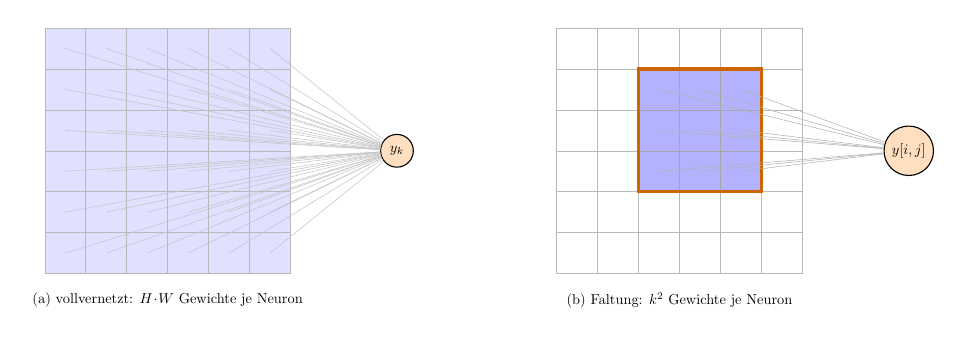
\begin{tikzpicture}[scale=0.52, every node/.style={transform shape}]
  % ---- Panel a: vollvernetzt ----
  \begin{scope}[shift={(0,0)}]
    \foreach \i in {0,...,5}{\foreach \j in {0,...,5}{
      \fill[blue!12] (\i,\j) rectangle ++(1,1);
      \draw[gray!55,very thin] (\i,\j) rectangle ++(1,1);}}
    \node (outa) at (8.6,3) [circle,draw,fill=orange!25,minimum size=8mm] {$y_k$};
    \foreach \i in {0,...,5}{\foreach \j in {0,...,5}{
      \draw[gray!45,very thin] (\i+0.5,\j+0.5) -- (outa);}}
    \node[below] at (3,-0.35) {(a) vollvernetzt: $H\!\cdot\!W$ Gewichte je Neuron};
  \end{scope}
  % ---- Panel b: Faltung ----
  \begin{scope}[shift={(12.5,0)}]
    \foreach \i in {0,...,5}{\foreach \j in {0,...,5}{
      \draw[gray!55,very thin] (\i,\j) rectangle ++(1,1);}}
    \foreach \i in {2,3,4}{\foreach \j in {2,3,4}{
      \fill[blue!30] (\i,\j) rectangle ++(1,1);
      \draw[gray!70,very thin] (\i,\j) rectangle ++(1,1);}}
    \draw[very thick,orange!80!black] (2,2) rectangle (5,5);
    \node (outb) at (8.6,3) [circle,draw,fill=orange!25,minimum size=8mm] {$y[i,j]$};
    \foreach \i in {2,3,4}{\foreach \j in {2,3,4}{
      \draw[gray!60,very thin] (\i+0.5,\j+0.5) -- (outb);}}
    \node[below] at (3,-0.35) {(b) Faltung: $k^2$ Gewichte je Neuron};
  \end{scope}
\end{tikzpicture}
\caption[Vollvernetzte Schicht gegen Faltungsschicht]{Lokale rezeptive Felder.
(a)~In einer vollvernetzten Schicht nach Gleichung~\eqref{eq:fc} ist jedes
Ausgabeneuron mit allen $H\cdot W$ Eingangspixeln verbunden. (b)~In einer
Faltungsschicht nach Gleichung~\eqref{eq:conv} beschränkt sich die Summation auf
eine $k\times k$-Nachbarschaft; für $k=3$ sinkt die Zahl der Verbindungen je
Ausgabeneuron bei $640\times640$ Eingabe von 409\,600 auf 9. Zugleich wird
derselbe Kernel an allen Positionen verwendet (Weight Sharing), sodass die
Parameterzahl der Schicht unabhängig von der Bildgröße wird.}
\label{abb:rezeptivesfeld}
\end{figure}

Die klassische statistische Lerntheorie führt hohe Parameterzahlen darüber
hinaus auf eine erhöhte Modellkapazität und damit auf eine Neigung zur
Überanpassung zurück \parencite[Kap.~5]{goodfellow2016}. Für tiefe neuronale
Netze ist dieser Zusammenhang allerdings nicht ungebrochen gültig:
\textcite{zhang2017rethinking} zeigen experimentell, dass gängige Faltungsnetze
zufällige Beschriftungen der Trainingsdaten vollständig memorieren können und
dennoch auf realen Daten gut generalisieren. Dies ist ein Befund, der die klassische
Kapazitätsargumentation als alleinige Erklärung in Frage stellt. Der belastbare
Vorteil lokaler rezeptiver Felder liegt daher weniger in einer Vermeidung von
Überanpassung an sich als in der beschriebenen Stichprobeneffizienz und im
deutlich reduzierten Rechenaufwand.

In einer Faltungsschicht wird die Summation stattdessen auf eine lokale
Nachbarschaft $\mathcal{N}_{k \times k}$ der Größe $k \times k$ beschränkt:
\begin{equation}
y[i,j] = \sigma\!\left(\sum_{(u,v)\in\mathcal{N}_{k\times k}} w[u,v]\,
x[i+u,\,j+v] + b\right)
\label{eq:conv}
\end{equation}

Die Anzahl der Verbindungen je Ausgabeneuron sinkt damit von $H \cdot W$ auf
$k^2$ -- für $k = 3$ von 409\,600 auf 9 (Abbildung~\ref{abb:rezeptivesfeld}).
Die Rechtfertigung liegt in der lokalen Korrelationsstruktur natürlicher Bilder:
Die Korrelation benachbarter Pixelwerte fällt mit wachsendem Abstand rasch
ab, sodass weit entfernte Pixel für lokale Merkmalsentscheidungen kaum
Information beitragen \parencite{lecun1998}.

Das theoretische rezeptive Feld wächst mit der Netztiefe. Bezeichnet $r_\ell$
seine Kantenlänge nach Schicht $\ell$, $k_\ell$ die Kernelgröße und $s_\ell$ die
Schrittweite, der Laufindex $m$ im Produkt bezeichnet dieselbe Größe für die jeweil
 vorangehenden Schichten, so gilt die Rekursion
\begin{equation}
r_\ell = r_{\ell-1} + (k_\ell - 1)\prod_{m=1}^{\ell-1} s_m,
\qquad r_0 = 1.
\label{eq:rf}
\end{equation}

Bei reinen $3\times3$-Faltungen mit $s_m = 1$ wächst $r_\ell$ lediglich linear
($r_\ell = 2\ell + 1$); erst durch Schrittweiten $s_m = 2$ wächst das Produkt
exponentiell, sodass das rezeptive Feld schnell große Bildbereiche umfasst.
Hieraus entsteht die in Abschnitt~\ref{sec:hierarchie} beschriebene
Merkmalshierarchie. Zu beachten ist, dass das \emph{effektive} rezeptive Feld
kleiner ausfällt als dieses theoretische Maß:
\textcite{luo2016} zeigen, dass der Einfluss
$\partial y_{\text{Zentrum}} / \partial x[i,j]$ annähernd gaußförmig zum Zentrum
hin abfällt und nur ein Bruchteil des theoretischen Felds tatsächlich zur
Ausgabe beiträgt.

\absatz{Geteilte Gewichte (Weight Sharing).} Ohne Gewichtsteilung besäße jede
Position $(i,j)$ einen eigenen Kernel $w_{ij}$, was auf $H \cdot W \cdot k^2$
Parameter je Merkmalskarte führte. Weight Sharing bedeutet formal, dass
$w_{ij} = w$ für alle $(i,j)$ gilt; die Schicht wird dadurch zur diskreten
Faltung (genauer: Kreuzkorrelation)
\begin{equation}
y[i,j] = (w * x)[i,j] = \sum_{u,v} w[u,v]\,x[i+u,\,j+v],
\end{equation}
mit lediglich $k^2$ Parametern je Kernel. Für eine Schicht mit $C_{\text{in}}$
Eingangs- und $C_{\text{out}}$ Ausgangskanälen ergeben sich
$C_{\text{out}} \cdot C_{\text{in}} \cdot k^2 + C_{\text{out}}$ Parameter --
unabhängig von der Bildgröße. Dies ist der entscheidende Unterschied zur
vollvernetzten Schicht, deren Parameterzahl mit $H \cdot W$ skaliert.

Die zentrale Eigenschaft ist die \textbf{Translationsäquivarianz}. Bezeichnet
$(T_\tau x)[i,j] = x[i-\tau_1,\,j-\tau_2]$ die Verschiebung um $\tau$, so gilt
für die Faltungsoperation $f$:
\begin{equation}
f(T_\tau x) = T_\tau f(x).
\label{eq:aequivarianz}
\end{equation}

Eine Verschiebung der Eingabe führt also zu einer identischen Verschiebung der
Ausgabe-Merkmalskarte. Die Rechtfertigung ist die (näherungsweise) Stationarität
natürlicher Bildstatistik: Die relevanten lokalen Merkmale sind ortsunabhängig,
eine Kante bleibt eine Kante, unabhängig von ihrer Position. Zu betonen ist,
dass Äquivarianz nicht Invarianz bedeutet. Diese entsteht erst durch das
nachfolgend beschriebene Subsampling.

Aus der Gewichtsteilung folgen drei praktische Konsequenzen: erstens eine
erhöhte Dateneffizienz, da ein Muster, das nur an wenigen Positionen in den
Trainingsdaten vorkommt, dennoch überall erkannt wird; zweitens eine
Einschränkung des Hypothesenraums, da die Nebenbedingung $w_{ij} = w$ nur noch
translationsäquivariante Abbildungen zulässt -- eine Beschränkung, die dem
tatsächlichen Charakter der Aufgabe entspricht und in diesem Sinne als
struktureller Prior wirkt; drittens die Notwendigkeit mehrerer Kernel je
Schicht, da ein Kernel genau ein Muster repräsentiert
\parencite{lecun1998,goodfellow2016}.

\absatz{Räumliches Subsampling.} Für die Objekterkennung ist häufig
\emph{Invarianz} gegenüber kleinen Verschiebungen erwünscht, also
$f(T_\tau x) \approx f(x)$ für kleine $\|\tau\|$. Diese entsteht durch
stufenweise Reduktion der räumlichen Auflösung -- klassisch durch Pooling über
ein Fenster $\mathcal{P}$ der Größe $p \times p$ mit Schrittweite $s$:
\begin{equation}
y[i,j] = \max_{(u,v)\in\mathcal{P}} x[s\cdot i + u,\; s\cdot j + v]
\qquad \text{(Max-Pooling)}
\end{equation}

In modernen Architekturen wie YOLO26 wird dieselbe Auflösungsreduktion
überwiegend durch Faltungen mit Schrittweite $s = 2$ realisiert. In beiden Fällen
bleibt lediglich erhalten, \emph{ob} ein Merkmal innerhalb des Fensters auftrat,
nicht seine exakte Position. Für Verschiebungen $\|\tau\|_\infty < p$ innerhalb
desselben Pooling-Fensters bleibt die Ausgabe unverändert
\parencite{lecun1998,goodfellow2016}.

Die Ausgabegröße nach einer Schicht mit Kernelgröße $k$, Schrittweite $s$ und
Randauffüllung $p_{\text{pad}}$ beträgt
\begin{equation}
H_{\text{out}} = \left\lfloor
\frac{H_{\text{in}} + 2p_{\text{pad}} - k}{s} \right\rfloor + 1,
\end{equation}
woraus für $s = 2$ näherungsweise eine Halbierung je Stufe folgt. Nach $L$
solchen Stufen beträgt die Gesamtschrittweite $S = \prod_{\ell} s_\ell = 2^L$;
die Zahl der räumlichen Positionen sinkt dabei um den Faktor $S^2$, was den mit
der Tiefe wachsenden Kanalzahlen entgegenwirkt.

Der Preis ist ein Verlust an Ortsinformation, der bei kleinen Objekten kritisch
wird. Eine Zelle der Merkmalsebene mit Gesamtschrittweite $S$ entspricht einem
Bildbereich von $S \times S$ Pixeln. Ein Objekt mit Durchmesser $d$ Pixeln
belegt dort nur $d/S$ Zellen; für $d < S$ ist es kleiner als eine einzelne Zelle
und kann strukturell nicht mehr zuverlässig lokalisiert werden. Konkret gilt für
z.B. die feinste Detektionsebene P3 in YOLO26 mit $S = 8$: Ein Rohrprofil mit $d = 6$ Pixeln
unterschreitet diese Grenze. Dieser Zusammenhang begründet sowohl die
Multi-Skalen-Fusion moderner Detektoren (Abschnitt~\ref{sec:neck}) als auch die
in Abschnitt~\ref{sec:anwendung} diskutierten Gegenmaßnahmen der erhöhten
Eingabeauflösung bzw.\ Kachelung, die beide $d$ relativ zu $S$ vergrößern.

\absatz{Zusammenspiel.} Die drei Prinzipien reduzieren die Parameterzahl in
aufeinander aufbauenden Schritten: Lokale rezeptive Felder senken die
Verbindungen je Neuron von $H \cdot W$ auf $k^2$, Weight Sharing eliminiert die
Abhängigkeit der Parameterzahl von der Bildgröße, und Subsampling reduziert die
Zahl der zu verarbeitenden Positionen um $S^2$ und erzeugt zugleich lokale
Translationsinvarianz. Gemeinsam kodieren sie genau jene Annahmen, die für
Bilddaten zutreffen: Lokalität, Stationarität und Toleranz gegenüber kleinen
Verschiebungen. \textcite{lecun1998} formulierten diese Prinzipien am Beispiel
der Architektur LeNet-5 zur Ziffernerkennung.

\subsection{Aufbau eines CNNs}

Ein typisches CNN besteht aus einer Abfolge folgender Schichttypen:

\absatz{Faltungsschichten (Convolutional Layers).} Kernstück des CNNs ist die
diskrete Faltungsoperation. Ein Filterkern (Kernel), typischerweise der Größe
$3\times3$ oder $5\times5$, wird über das Eingabebild bzw.\ die Merkmalskarte
(Feature Map) geschoben. An jeder Position wird das Skalarprodukt zwischen
Kernelgewichten und dem darunterliegenden Bildausschnitt berechnet. Das Ergebnis
ist eine neue Merkmalskarte, die angibt, wie stark das vom Kernel
repräsentierte Muster an der jeweiligen Position ausgeprägt ist. Die Gewichte der
Kernel werden nicht manuell festgelegt, sondern im Training mittels
Backpropagation gelernt \parencite{lecun1998,goodfellow2016}.

\absatz{Aktivierungsfunktionen.} Auf jede Faltung folgt eine nichtlineare
Aktivierungsfunktion, ohne die das Netz nur lineare Abbildungen lernen könnte.
In modernen CNNs hat sich die Rectified Linear Unit (ReLU),
$f(x) = \max(0, x)$, sowie deren Varianten (z.\,B.\ SiLU/Swish) durchgesetzt, da
sie das Problem verschwindender Gradienten abmildert und effizient zu berechnen
ist \parencite{krizhevsky2012}.

\absatz{Pooling-Schichten.} Pooling-Operationen (meist Max-Pooling) reduzieren
die räumliche Auflösung der Merkmalskarten, indem sie z.\,B.\ aus jedem
$2\times2$-Bereich nur den Maximalwert übernehmen. Dies verringert den
Rechenaufwand, vergrößert das rezeptive Feld nachfolgender Schichten und sorgt
für eine gewisse Robustheit gegenüber kleinen Verschiebungen
\parencite{goodfellow2016}.

\absatz{Vollvernetzte Schichten (Fully Connected Layers).} Am Ende klassischer
CNN-Architekturen fassen vollvernetzte Schichten die extrahierten Merkmale
zusammen und bilden sie z.\,B.\ auf Klassenwahrscheinlichkeiten ab. In modernen
Detektionsarchitekturen werden sie zunehmend durch faltungsbasierte
Prädiktionsköpfe ersetzt.

\subsection{Merkmalshierarchie und Objektdetektion}
\label{sec:hierarchie}

Auf jede Faltung folgt eine nichtlineare Aktivierung -- heute überwiegend die
Rectified Linear Unit $f(x) = \max(0,x)$ oder Varianten wie SiLU
\parencite{krizhevsky2012} --, ohne die das Netz nur lineare Abbildungen lernen
könnte. Aus der Stapelung entsteht ein hierarchischer Aufbau der
Repräsentationen: Frühe Schichten reagieren auf Kanten und Farbverläufe, mittlere
auf Texturen und Teilstrukturen, tiefe auf semantische Objektbestandteile
\parencite{zeiler2014}. Diese datengetriebene Merkmalsextraktion tritt an die
Stelle des manuell entworfenen Feature Engineering und gilt als wesentlicher
Grund für die Leistungssprünge tiefer Netze \parencite{lecun2015}. Am Ende
klassischer Architekturen fassen vollvernetzte Schichten die Merkmale zusammen;
in modernen Detektoren sind sie vollständig durch Faltungen ersetzt
(Abschnitt~\ref{sec:neck}). Residualverbindungen \parencite{he2016} ermöglichen
das stabile Training sehr tiefer Netze und sind Standardbaustein nahezu aller
CNN-Backbones.

Für diese Arbeit ist nicht die Klassifikation relevant, sondern die
\textbf{Objektdetektion}: das gleichzeitige Lokalisieren und Klassifizieren
mehrerer Objekte. Zweistufige Detektoren erzeugen zunächst Regionsvorschläge und
klassifizieren diese anschließend \parencite{ren2015}; einstufige Detektoren
formulieren die Detektion als einmaliges Regressionsproblem und sagen in einem
Durchlauf direkt Boxen und Klassenwahrscheinlichkeiten vorher
\parencite{redmon2016,liu2016ssd}, was Echtzeitfähigkeit bei geringen
Genauigkeitseinbußen ermöglicht. Klassisch nachgeschaltet ist die
Non-Maximum Suppression (NMS), die redundante überlappende Detektionen anhand
ihrer Intersection over Union unterdrückt -- bei dicht gepackten gleichartigen
Objekten eine potenzielle Fehlerquelle.

\section{YOLO26}
\label{sec:yolo26}

\subsection{Einordnung und Neuerungen}

\enquote{You Only Look Once} wurde 2016 als erster echtzeitfähiger einstufiger
Detektor vorgestellt \parencite{redmon2016}; ab YOLOv8 übernahm Ultralytics die
Weiterentwicklung und etablierte ankerfreie, entkoppelte Detektionsköpfe
\parencite{sapkota2025}. YOLO26 wurde im September 2025 vorgestellt und
unterscheidet sich von YOLO11 durch vier koordinierte Änderungen: ein
Dual-Head-Design für NMS-freie Inferenz, den Wegfall der Distribution Focal Loss,
ProgLoss zusammen mit STAL sowie den MuSGD-Optimierer
\parencite{ultralytics2026,sapkota2025}.

Für diese Arbeit ist davon eine Änderung einschlägig: Die
\emph{Small-Target-Aware Label Assignment} garantiert positive Labelzuweisungen
auch für sehr kleine Objekte -- genau das Problem klassischer
Zuweisungsstrategien, das Abschnitt~\ref{sec:p2} quantifiziert.

\subsection{Backbone, Neck, Head und die Merkmalspyramide}
\label{sec:neck}

YOLO26 folgt der Dreiteilung \textbf{Backbone $\to$ Neck $\to$ Head}. Das
Backbone reduziert die räumliche Auflösung stufenweise per Stride-2-Faltungen
($1024 \to 512 \to 256 \to 128 \to 64 \to 32$ bei $1024$\px{} Eingabe), während
die Kanalzahl wächst -- räumliche Präzision wird gegen semantische Tiefe
getauscht. Jeder Faltung folgen Batch-Normalisierung und SiLU-Aktivierung; die
Blöcke sind im CSP-Stil mit Residualverbindungen organisiert, am Ende aggregiert
ein SPPF-Modul Kontext über mehrere Pooling-Größen.

\absatz{Neck.} Das Neck verbindet die Auflösungsstufen in beide Richtungen
(FPN/PAN-Prinzip, \cite{lin2017fpn}): Tiefe, semantisch reiche Merkmalskarten
werden hochskaliert und mit den feinen, ortsgenauen Karten früherer Stufen
zusammengeführt, und umgekehrt. Der Head erhält dadurch mehrere Ausgabeebenen,
die nach Objektgröße zuständig sind. Die Standardkonfiguration liefert drei
Ebenen P3/P4/P5 mit den Gesamtschrittweiten 8/16/32; zusätzlich existiert eine
Konfiguration mit einer vierten, feineren Ebene \textbf{P2 mit Schrittweite~4}
(Abbildung~\ref{abb:pyramide}). Sie ist der Gegenstand von
Abschnitt~\ref{sec:p2}.

\begin{figure}[htbp]
\centering
\begin{tikzpicture}[x=1cm,y=1cm]
  % ---- Merkmalsebenen als Quadrate, Seitenlaenge proportional zur Gittergroesse
  \draw[fill=red!8,dashed,thick,red!60!black] (0,0) rectangle (4,4);
  \draw[step=0.5,gray!35,very thin] (0,0) grid (4,4);
  \draw[fill=blue!8] (4.7,0) rectangle (6.7,2);
  \draw[step=0.5,gray!35,very thin] (4.7,0) grid (6.7,2);
  \draw[fill=blue!8] (7.4,0) rectangle (8.4,1);
  \draw[step=0.5,gray!35,very thin] (7.4,0) grid (8.4,1);
  \draw[fill=blue!8] (9.1,0) rectangle (9.6,0.5);

  \node[below,align=center,font=\scriptsize] at (2,-0.2)
       {\textbf{P2} $\;$ Stride 4\\$256\times256$\\65\,536 Positionen};
  \node[below,align=center,font=\scriptsize] at (5.7,-0.2)
       {\textbf{P3} $\;$ Stride 8\\$128\times128$\\16\,384};
  \node[below,align=center,font=\scriptsize] at (7.9,-0.2)
       {\textbf{P4} $\;$ 16\\$64^2$\\4\,096};
  \node[below,align=center,font=\scriptsize] at (9.35,-0.2)
       {\textbf{P5} $\;$ 32\\$32^2$\\1\,024};

  \node[above,font=\scriptsize,red!60!black,align=center] at (2,4.15)
       {\emph{nur in der Variante} \code{-p2}};
  \node[above,font=\scriptsize,align=center] at (7.0,4.15)
       {Standardkonfiguration P3--P5};
  \draw[decorate,decoration={brace,amplitude=4pt},gray!60!black]
       (4.7,4.05) -- (9.6,4.05);
  \node[font=\scriptsize,align=left,anchor=west] at (10.1,2.6)
       {kleine\\Objekte};
  \node[font=\scriptsize,align=left,anchor=west] at (10.1,1.2)
       {große\\Objekte};
  \draw[-{Latex[length=1.6mm]},gray!60!black] (10.35,2.3) -- (10.35,1.6);
\end{tikzpicture}
\caption[Merkmalsebenen des Detektionskopfes]{Merkmalsebenen des
Detektionskopfes bei einer Eingabe von $1024\times1024$ Pixeln. Die
Seitenlänge der Quadrate ist proportional zur Gittergröße. Jede Zelle einer
Ebene mit Schrittweite $S$ entspricht einem Bildbereich von $S \times S$ Pixeln
und sagt Boxkoordinaten sowie Klassen-Scores vorher. Die Standardkonfiguration
nutzt P3--P5; die Variante \code{-p2} ergänzt die Ebene P2 mit Schrittweite~4,
die allein mehr Prädiktionspositionen enthält als P3, P4 und P5 zusammen.}
\label{abb:pyramide}
\end{figure}

\absatz{Head.} Das ursprüngliche YOLOv1 endete in zwei vollvernetzten Schichten
\parencite{redmon2016}, die den überwiegenden Teil aller Parameter enthielten,
die Eingabegröße fixierten und die räumliche Struktur zerstörten. Moderne
YOLO-Architekturen sind dagegen vollständig faltungsbasiert: Der Kopf besteht aus
kleinen Faltungsstapeln, die in $1\times1$-Faltungen münden. Eine
$1\times1$-Faltung ist mathematisch äquivalent zu einer vollvernetzten Schicht
über die Kanaldimension, wird aber \textbf{positionsgeteilt} angewendet --
dieselbe Operation verarbeitet die Kanäle jeder Gitterzelle separat. Das erhält
die Translationsäquivarianz bis in die Ausgabeschicht und macht das Netz
unabhängig von einer festen Eingabegröße. Der Kopf ist zusätzlich
\emph{entkoppelt} (getrennte Zweige für Klassifikation und Boxregression) und
\emph{ankerfrei}: Jede Gitterzelle regressiert direkt die Abstände zu den vier
Boxrändern. Damit ist die Zahl der Gitterzellen -- und nicht die Zahl der
Ankerboxen -- die Größe, die bestimmt, wie fein Objekte überhaupt aufgelöst
werden können.

\section{Anwendung auf die Zählung gestapelter Bauzäune}
\label{sec:anwendung}

Ein YOLO-Modell wird per Transfer Learning von COCO-vortrainierten Gewichten
\parencite{yosinski2014} auf eine einzige Objektklasse feinabgestimmt; die
Zaunanzahl ergibt sich aus der Zahl der detektierten Stirnflächen. Die
hierarchische Merkmalsextraktion des Backbones ist dafür gut geeignet:
Kreisförmige Metallprofile mit charakteristischem Hell-Dunkel-Verlauf sind
visuell einfache, texturarme Objekte, die bereits mittlere Netzschichten
repräsentieren können. YOLO26 adressiert die kritischen Eigenschaften des
Problems konzeptionell direkt: STAL und ProgLoss verbessern die Erkennung kleiner
Objekte, und die NMS-freie Inferenz eliminiert einen bei dicht gepackten
gleichartigen Objekten systematisch fehleranfälligen Hyperparameter -- ein zu
niedriger IoU-Schwellwert unterdrückt korrekte Detektionen benachbarter Rohre
(Unterzählung), ein zu hoher lässt Duplikate zu (Überzählung). Da es sich um ein
Ein-Klassen-Problem mit geometrisch einfachen Objekten handelt, genügen kleine
Modellvarianten. Anders als dichtebasierte Zählverfahren
\parencite{lempitsky2010,zhang2016counting} liefert die detektionsbasierte
Zählung pro Objekt eine sichtbare Box; Fehlzählungen sind damit lokalisierbar und
im Einsatz korrigierbar.

Drei Grenzen sind kritisch. Erstens die \textbf{Auflösung}: Die
Standard-Eingabegröße von $640\times640$ ist für diese Aufgabe zu klein -- wird
eine hochaufgelöste Stapelaufnahme darauf herunterskaliert, schrumpfen die
Profile auf wenige Pixel und unterschreiten die Auflösungsgrenze der P3-Ebene.
Abhilfe schaffen eine erhöhte Eingabeauflösung (Rechenaufwand wächst
quadratisch), eine Kachelung des Bildes \parencite{akyon2022sahi} oder ein
feinerer Detektionskopf (Abschnitt~\ref{sec:p2}). Zweitens die
\textbf{Verdeckung}: Verkippte Zäune verdecken benachbarte Profile, und visuell
ähnliche Strukturen -- Gitterknoten, Löcher im Maschendraht, Schattenspalten --
drohen als Falschpositive. Drittens der \textbf{Datenbedarf}: Ein eigener
annotierter Datensatz ist unumgänglich und muss die reale Varianz abdecken. Genau
hier setzt der Praxisteil an -- die Domänenlücke wird nicht durch Handannotation
geschlossen, sondern durch eine Synthese-Pipeline, deren Entwurf Gegenstand der
Kapitel~\ref{kap:augtheorie} bis \ref{kap:trainingszeit} ist.
